\section{Clase 4 - Pr\'actica 2 (Ecuaciones diferenciales - Problema de valores iniciales)}

\subsection{Errores de truncado}

\underline{Definici\'on}: Dados $x^{*},\ h$, definimos el error de truncado local $\tau = \tau(x^{*})$ como:

$$y(x^{*} + h) = y(x^{*}) + h\phi(x^{*}, y(x^{*}), h) + h\tau$$

\textit{Ejemplo}: Si $\theta \in (x^{*}, x^{*} + h)$

\begin{itemize}
	\item Para Euler: $\tau = \frac{h}{2}y''(\theta)$
	
	\item Para Taylor de orden $k$: $\tau = \frac{h^{k}}{(k + 1)!}y^{k + 1}(\theta)$
\end{itemize}

\underline{Definici\'on}: Decimos que el m\'etodo de un paso tiene orden $p \in \mathbb{N}$ si $\tau = \mathcal{O}(h^{p})$, si suponemos que la soluci\'on tiene derivada de orden $p + 1$ acotada.\\

Euler es un m\'etodo de orden 1, Taylor 2 o RK2 son de orden 2, etc.\\

\underline{Definici\'on}: Decimos que el m\'etodo de un paso $y_{i + 1} = y_{i} + h\phi(x_{i}, y_{i}, h)$ converge si para cualquier $x^{*} \in [a, b],\ \lim \limits_{h \rightarrow \infty} y_{n} = y(x^{*})$.\\

\underline{Definici\'on}: Condici\'on CL. Decimos que $\phi(x, y, h)$ satisface la condici\'on CL si:

$$|\phi(x, u, h) - \phi(x, v, h)| \leq K|u - v|$$

con $x \in [a, b],\ 0 \leq h \leq b - a,\ u, v \in \mathbb{R}$. Luego, $\phi$ es Lipschitz respecto de su segunda variable.\\

\underline{Teorema}: Error global. Si $\phi$ satisface la condici\'on CL con constante $K$ y adem\'as $h = \frac{b - a}{n},\ x_{j} = a + hj,\ j = 0, \cdots, n$, entonces:

$$|E_{j}| = |y(x_{j}) - y_{j}| \leq \frac{\tau_{\max}}{K}(e^{K(x_{j} - x_{0})} - 1)$$

donde $\tau_{\max} = \max \limits_{0 \leq i \leq j} |\tau_{i}|$.\\

\underline{Demostraci\'on}:

$$y_{j + 1} = y_{j} + h\phi(x_{j}, y_{j}, h)$$

$$y(x_{j + 1}) = y(x_{j}) + h\phi(x_{j}, y_{j}(x_{j}), h) + h\tau_{j}$$

$$|E_{j + 1}| = |y(x_{j + 1}) - y_{j + 1}| = |y(x_{j}) - y_{j} + h\phi(x_{j}, y(x_{j}), h) - h\phi(x_{j}, y_{j}, h) + h\tau_{j}|$$

$$\leq |E_{j}| + h|\phi(x_{j}, y(x_{j}), h) \phi(x_{j}, y_{j}, h)| + h|\tau_{j}| \leq |E_{j}| + hK|E_{j}| + h\tau_{\max} = (1 + hK)|E_{j}| + h\tau_{\max}$$

$$\leq (1 + hK)[(1 + hK)|E_{j - 1}| + h\tau_{\max}] + h\tau_{\max} = (1 + hK)^{2}E_{j - 1} + (1 + hK)h\tau_{\max} + h\tau_{\max}$$

$$\leq (1 + hK)^{j + 1}|E_{j - 1}| + h\tau_{\max}\sum \limits_{l = 0}^{j} (1 + hK)^{l} = h\tau_{\max} \frac{(1 + hK)^{j + 1} - 1}{hK} = \frac{\tau_{\max}}{K}[(1 + hK)^{j - 1} - 1]$$

Como vale que $(1 + z)^{n} \leq e^{nz},\ z \in \mathbb{R}_{\geq 0}$, luego:

$$\frac{\tau_{\max}}{K}[(1 + hK)^{j - 1} - 1] \leq \frac{\tau_{\max}}{K}(e^{hK(j + 1)} - 1)$$

Caso particular: $|y_{N} - y_{0}| \leq \frac{\tau_{\max}}{K}(e^{K(x_{N} - x_{0})} - 1)$\\

C\'omo ver el orden de los m\'etodos en forma num\'erica?

$$E = \mathcal{O}(h^{p}) \approx \text{Error} = ch^{p}$$

$$\Rightarrow \log(\text{Error}) = \log(ch^{p}) = \log(c) + \log(h^{p}) = k + p\log(h) \Rightarrow y = k + px$$

El orden se ve como la pendiente de una recta.\\

\underline{Euler}: $\phi(x_{i}, y_{i}, h) = f(x_{i}, y_{i})$\\

La constante $K$ del teorema es la constante de Lipschitz de $f(x, y)$, $|f(x, u) - f(x, v)| \leq K|u - v|$

$$\tau_{i} = \frac{h}{2}y''(\theta)$$

es el error de truncado local para Euler, con $\theta \in (x_{i}, x_{i + 1})$.\\

Como $y' = f(x, y) \Rightarrow y'' = f'(x, y) = f_{x}(x, y) + f_{y}(x, y)y' = f_{x}(x, y) + f_{y}(x, y)f(x, y)$.\\

Sea $Y = \max \limits_{x \in [x_{0}, x_{N}]} |y''(x)| \Rightarrow |E_{N}| \leq \frac{h}{2K}Y(e^{K(x_{N} - x_{0})} - 1)$,

$$|y_{N} - y(x^{*})| \leq \frac{(x^{*} - a)}{2Kn}Y(e^{K(x_{N} - x_{0})} - 1) \rightarrow_{n \rightarrow +\infty} 0$$

Para que converja, $\tau$ tiene que tener un $h$. El m\'etodo de un paso converge si $\tau \rightarrow_{h \rightarrow 0} 0$.\\

\underline{Definici\'on}: Se dice que el m\'etodo de un paso es consistente si el error de truncado local $\tau \rightarrow_{h \rightarrow 0} 0$.\\

Ver consistencia es equivalente a ver que $\phi$ (continua en $h$) satisface $\phi(x_{i}, y(x_{i}), 0) = f(x_{i}, y(x_{i}))$. Lo que propongo como esquema aproxima a mi ecuaci\'on diferencial.\\

Para los m\'etodos de un paso, la consistencia implica la convergencia (por teorema): $\tau_{\max} \rightarrow_{h \rightarrow 0} 0$, entonces converge.\\

\textit{Ejemplo}: Considerar el problema de valores iniciales en $[0, 1]$:

$$ 
	\begin{cases}
        y'(t) = t\cos^{2}(y(t))\\
        y(0) = 5\\
    \end{cases}
$$

\begin{itemize}
	\item a) Escribir la iteraci\'on del m\'etodo de Euler correspondiente a este problema.
	
	$$ 
		\begin{cases}
        	y_{i + 1} = y_{i} + hf(t_{i}, y_{i})\\
        	y_{0} = 5\\
    	\end{cases}
	\Rightarrow
		\begin{cases}
        	y_{i + 1} = y_{i} + h(t_{i}\cos^{2}(y_{i}))\\
        	y_{0} = 5\\
    	\end{cases}
	$$
		
	con $0 \leq i \leq N - 1,\ h = \frac{t_{N} - t_{0}}{N} = \frac{1}{N}$\\
	
	\item b) Hallar $h$ para que el error al estimar $y(1)$ con el m\'etodo de Euler sea menor que $10^{-3}$.
	
	$$|y_{N} - y(1)| \leq \frac{\tau_{\max}}{K}(e^{K(1 - 0)} - 1)$$
	
	$\phi(t_{i}, y_{i}, h) = f(t, y) = t\cos^{2}(y)$. Quiero hallar $K$:
	
	$$|f(t, x) - f(t, y)| \leq K|x - y| \Rightarrow |t\cos^{2}(x) - t\cos^{2}(y)| = \bigg| \frac{\partial f}{\partial y}(t, \theta)\bigg||x - y| = |t2\cos(\theta)\sin(\theta)||x - y| \leq 2|x - y|$$
	
	Luego, $K = 2$ y nos queda:
	
	$$|y_{N} - y(1)| \leq \frac{\tau_{\max}}{2}(e^{2} - 1)$$

	En Euler, $|\tau_{i}| = \frac{h}{2}|y''(\theta)|,\ \theta \in (t_{i}, t_{i + 1})$. Hay dos formas de hallar esta derivada segunda:
	
	$$1^{\circ})\ y''(t) = 1\cos^{2}(y(t)) + t2\cos(y(t))(-\sin(y(t)))y'(t) = \cos^{2}(y(t)) - 2t\cos(y(t))\sin(y(t))t\cos^{2}(y(t))$$
	
	$$2^{\circ})\ y''(t) = \cos^{2}(y) + t2\cos(y)(-\sin(y))t\cos^{2}(y) = \frac{\partial f}{\partial t} + \frac{\partial f}{\partial y}f(t, y)$$

	Si acotamos $y''(t)$:
	
	$$|y''(t)| \leq |\cos^{2}(y)| + 2t^{2}|\cos^{3}(y)||\sin(y)| \leq 1 + 2 = 3$$
	
	pues $t \in [0, 1]$. Luego, $|\tau_{i}| \leq \frac{3}{2}h$, entonces:
	
	$$|y_{N} - y(1)| \leq \frac{3}{2}h\frac{1}{2}(e^{2} - 1) \leq 10^{-3}$$
	
	$$\Rightarrow h \leq \frac{10^{-3}}{6}$$
\end{itemize}

\textit{Python}: Euler

$$ 
	\begin{cases}
        y'(t) = y(t),\ t \in [0, 1]\\
        y(0) = 1\\
    \end{cases}
$$

\begin{verbatim}
	import numpy as np
	import matplotlib.pyplot as plt
	
	def f(t, y):
	    return y
		
	def Euler(a, b, f, y0):
	    h = [0.1, 0.0625, 0.05, 0.025, 0.01]
	    m = len(h)
	    logH = np.log(h)
	    ExactaEnUno = np.exp(1)
	    E = np.zeros(m)
		
	    for j in range(0, m):
	        N = int((b - a) / h[j])
	        t = np.linspace(a, b, N + 1)
	        y = np.zeros(N + 1)
	        y[0] = 1
	        
	        for i in range(0, N):
	            y[i + 1] = y[i] + h[j] * f(t[i], y[i])
	            
	        plt.plot(t, y)
	        AproxEnUno = y[N]
	        
	        E[j] = np.abs(ExactaEnUno - AproxEnUno)
	        
	    logE = np.log(E)
	    
	    Pendiente = np.abs((logE[m - 2] - logE[m - 1]) / (logH[m - 2] - logH[m - 1]))
		
	    return Pendiente
		
	a = 0
	b = 1
	y0 = 1
	
	Pendiente = Euler(a, b, f, y0)
	
	print(Pendiente)
	# 0.9852497002053401
\end{verbatim}

\begin{figure}[H]
  \centering
  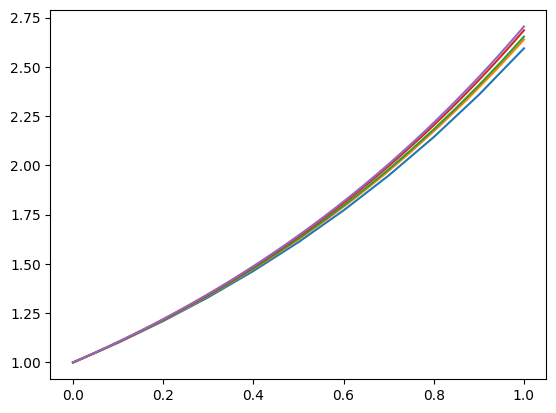
\includegraphics[width=0.6\linewidth]{Clase4_Practica2/euler_c4p2.png}
\end{figure}